\documentclass{beamer}
\usepackage{amsmath, amssymb}
\usepackage{physics}
\usepackage{subfig}
\usepackage{hyperref}
%\usepackage{verbatim}

\usepackage[utf8]{inputenc}
\usetheme{Madrid}

\title{Usage of JEWEL generator}
\author{Jinghong Yang}

\AtBeginSection[]
{
  \begin{frame}
    \frametitle{Table of Contents}
    \tableofcontents[currentsection]
  \end{frame}
}

\begin{document}

\begin{frame}
\titlepage
\end{frame}

\begin{frame}
\frametitle{Table of Contents}
\tableofcontents
\end{frame}

\section{Installation}
\begin{frame}
 \frametitle{Installing prerequisites}

 \begin{figure}[h]
  \centering
  \href{https://jewel.hepforge.org/gettingstarted.html}{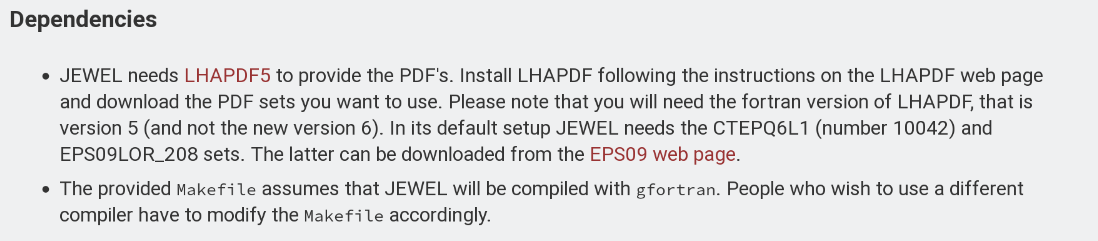
\includegraphics[width=0.9\linewidth]{dependencies.png}}
 \end{figure}

 \begin{block}{Download and Install LHAPDF5}
 \begin{scriptsize}
  \url{https://lhapdf.hepforge.org/downloads?f=old}
  \url{https://lhapdf.hepforge.org/lhapdf5/install}
  \end{scriptsize}
 \end{block}

 \begin{exampleblock}{\href{https://lhapdf.hepforge.org/lhapdf5/manual\#tth_sEcA}{Download PDF sets (e.g. 5.9.1)} }
 \begin{scriptsize}
  \url{https://lhapdf.hepforge.org/downloads/?f=pdfsets/5.9.1/EPS09LOR_208.LHgrid}
  \url{https://lhapdf.hepforge.org/downloads?f=pdfsets/5.9.1//cteq6ll.LHpdf}\\
\end{scriptsize}
\begin{footnotesize}
Put them in (lhapdf path)\textit{/share/lhapdf/PDFsets/}
\end{footnotesize}
\end{exampleblock}

\begin{tiny}
\href{https://www.jyu.fi/science/en/physics/research/highenergy/urhic/npdfs/eps09}{alternative}
\end{tiny}


\end{frame}

\begin{frame}
 \frametitle{Compiling JEWEL}
 \begin{block}{Modify Makefile}
 LHAPDF\_PATH := (your lhapdf install path)/lib/
 \end{block}

 \begin{exampleblock}{Modifying your .bashrc or .zshrc}
 export LD\_LIBRARY\_PATH=/.../lhapdf-5.x.y/lib:\$LD\_LIBRARY\_PATH
 export LHAPATH=/.../lhapdf-5.x.y/share/lhapdf/PDFsets
 \end{exampleblock}
\end{frame}


\section{Data generation}
\begin{frame}
\frametitle{Run JEWEL}
\begin{itemize}
 \item Now you have two binaries: jewel-2.2.0-vac and jewel-2.2.0-simple
 \item ./jewel-2.2.0-vac $\langle$configuration file$\rangle$
 \item ./jewel-2.2.0-simple $\langle$configuration file$\rangle$
 \item \href{https://arxiv.org/pdf/1311.0048.pdf}{Documentation}
 \item The log file and output file are specified by the config file.
\end{itemize}

\begin{alertblock}{Caution}
Watch out for xsecs.dat, pdf.dat, and splitint.dat

If you change physical parameters, delete these files before you run JEWEL again.
\end{alertblock}



\end{frame}

\section{Generate gluon and quark jets}

\begin{frame}
 \begin{itemize}
  \item Show routine initpythia in jewel-2.2.0.f (roughly line 800)
  \item \href{https://pythia.org/download/pythia6/lutp0613man2.pdf}{Pythia 6 Documentation} (See pages 140, 145, and 195)
 \end{itemize}

 \begin{columns}

  \column{0.4\linewidth}
  \begin{exampleblock}{Gluons}
MSEL=0 \\
MSUB(13)=1\\
MSUB(68)=1\\
\phantom{Place holder MSUB}
  \end{exampleblock}

  \column{0.4\linewidth}
  \begin{block}{Quarks}
MSEL=0\\
MSUB(11)=1\\
MSUB(12)=1\\
MSUB(53)=1
  \end{block}


 \end{columns}


\end{frame}


\section{Data processing using RIVET}

\begin{frame}
 \frametitle{How to understand HepMC2 ascii format}
 \begin{itemize}
  \item \href{http://hepmc.web.cern.ch/hepmc/releases/HepMC2_user_manual.pdf}{Documentation link}
  \item Reminder to myself: show an example
  \item Use Rivet
 \end{itemize}

\begin{exampleblock}{Rivet usage}
	rivet \textit{(hepmc file)} -a \textit{(analysis name)}\\
	rivet output.hepmc -a MC\_JETS\\
	\phantom{Placeholder}\\
	For Jewel outputs, use\\
	rivet --ignore-beams output.hepmc -a MC\_JETS
\end{exampleblock}

\begin{alertblock}{Warning}
	Rivet 3.1.5 and above seems to be incompatible with JEWEL.
\end{alertblock}

\end{frame}  


\begin{frame}
 \frametitle{Rivet installation}
 % mention apptainer vs native install vs docker
 \begin{block}{Native install using bootstrap script}
 	\begin{scriptsize}
 	\url{https://gitlab.com/hepcedar/rivet/-/blob/release-3-1-x/doc/tutorials/installation.md}  \\
 \end{scriptsize}
 	Execute the bootstrap to install rivet and all its dependencies.
 \end{block}
However, the recommended way is to use Docker.

\begin{alertblock}{Hoffman2} 
	\begin{small}
	On Hoffman2 cluster, due to security concerns, apptainer is used instead of Docker.
	Apptainer (formerly named Singularity) is compatible with Docker container format.\\
	\emph{module load apptainer}
	\end{small}
\end{alertblock}

\begin{exampleblock}{Use apptainer/docker to install Rivet}
	   docker pull hepstore/rivet:3.1.4 \\
	   apptainer pull docker://hepstore/rivet:3.1.4
\end{exampleblock}

\end{frame}



\begin{frame}
 \frametitle{Using apptainer or docker}
 \begin{block}{Docker}
 
   	docker run -i --rm hepstore/rivet:3.X.Y (command)
   	
   	docker run -i  --rm  -v \$PWD:\$PWD -w \$PWD -u \`{}id -u \$USER\`{}:\`{}id -g\`{} hepstore/rivet:3.1.4 rivet output.hepmc -a MC\_JETS

%   	To make container read your files: \begin{footnotesize}-v \$PWD:\$PWD -w \$PWD -u \`{}id -u \$USER\`{}:\`{}id -g\`{} \end{footnotesize}
 \end{block}

\begin{exampleblock}{apptainer}
	apptainer exec (container image path)/rivet\_3.X.Y.sif (command)
	apptainer exec (path...)/rivet\_3.1.4.sif rivet output.hepmc -a MC\_JETS
\end{exampleblock}

Reminder to self: show how to use apptainer

\end{frame}


\begin{frame}
	\frametitle{To make life easier}
	\begin{block}{\href{https://gitlab.com/hepcedar/rivet/-/blob/release-3-1-x/doc/tutorials/docker.md\#running-rivet-through-docker}{Docker}}
%		alias rivet=\textquotesingle docker run -i  --rm  -u \`{}id -u \$USER\`{}:`{}id -g\`{}  -v \$PWD:\$PWD -w \$PWD  hepstore/rivet:X.Y.Z rivet\textquotesingle\\
%		alias rivet-mkanalysis=\textquotesingle docker run -i  --rm  -u \`{}id -u \$USER\`{}:`{}id -g\`{}  -v \$PWD:\$PWD -w \$PWD  hepstore/rivet:X.Y.Z rivet-mkanalysis\textquotesingle
%		alias rivet-buildplugin=\textquotesingle docker run -i  --rm  -u \`{}id -u \$USER\`{}:`{}id -g\`{}  -v \$PWD:\$PWD -w \$PWD  hepstore/rivet:X.Y.Z rivet-buildplugin\textquotesingle
%		alias rivet-mkhtml=\textquotesingle docker run -i  --rm  -u \`{}id -u \$USER\`{}:`{}id -g\`{}  -v \$PWD:\$PWD -w \$PWD  hepstore/rivet:X.Y.Z rivet-mkhtml\textquotesingle
%		alias yodamerge=\textquotesingle docker run -i --rm  -u \`{}id -u \$USER\`{}:`{}id -g\`{}  -v \$PWD:\$PWD -w \$PWD  hepstore/rivet:X.Y.Z yodamerge\textquotesingle
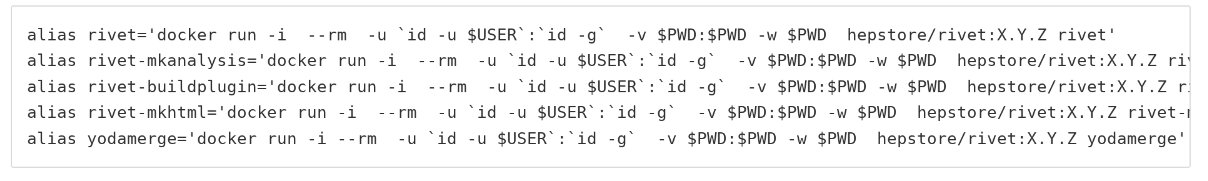
\includegraphics[width=\linewidth]{dockerAlias.png}
		
	\end{block}

	\begin{exampleblock}{Apptainer}
		alias rivet=\textquotesingle apptainer exec \textit{(path)}/rivet\_3.X.Y.sif rivet\textquotesingle \\
		alias rivet-mkhtml=\textquotesingle apptainer exec \textit{(path)}/rivet\_3.X.Y.sif rivet-mkhtml\textquotesingle \\
		alias rivet-build=\textquotesingle apptainer exec \textit{(path)}/rivet\_3.X.Y.sif rivet-build\textquotesingle \\
		alias yodamerge=\textquotesingle apptainer exec \textit{(path)}/rivet\_3.X.Y.sif yodamerge\textquotesingle \\
	\end{exampleblock}
\end{frame}
% if have time, talk a little bit more about native install

% mention jewel mkfifo
\begin{frame}
 \frametitle{Using named pipe}
 The HepMC file can get really large.
 
 Use named pipe to save space.
 \begin{exampleblock}{mkfifo}
 	\# suppose the output name is output.hepmc \\
 	mkfifo output.hepmc\\
 	./jewel-2.2.0-simple configuration.dat \& \\
 	rivet --ignore-beams output.hepmc -a \textit{Some\_analysis}
 \end{exampleblock}
\end{frame}


%\section{Troubleshooting}

\end{document}


